
% ----------------------------------------------------------------------
%  Set the document class
% ----------------------------------------------------------------------
\documentclass[11pt,a4paper,twoside]{article}

% ----------------------------------------------------------------------
% Define external packages, language, margins, fonts and new commands
% ----------------------------------------------------------------------
%\input{preamble} 
\usepackage[utf8]{inputenc}   % <<<<< Linux
\usepackage[english]{babel} % <<<<< English
\usepackage{notoccite}
\usepackage[skip=0.5\baselineskip]{caption}
\hyphenation{GTKWave}
\usepackage{listings}
\usepackage[all]{nowidow}

%blind text
\usepackage{lipsum}

\usepackage{graphicx}
\graphicspath{{./}{../../figlib/}{../mat/}{../sim/}}
\def\FontLn{% 16 pt normal
  \usefont{T1}{phv}{m}{n}\fontsize{16pt}{16pt}\selectfont}
\def\FontLb{% 16 pt bold
  \usefont{T1}{phv}{b}{n}\fontsize{16pt}{16pt}\selectfont}
\def\FontMn{% 14 pt normal
  \usefont{T1}{phv}{m}{n}\fontsize{14pt}{14pt}\selectfont}
\def\FontMb{% 14 pt bold
  \usefont{T1}{phv}{b}{n}\fontsize{14pt}{14pt}\selectfont}
\def\FontSn{% 12 pt normal
  \usefont{T1}{phv}{m}{n}\fontsize{12pt}{12pt}\selectfont}

% Use Arial font as default
%
\renewcommand{\rmdefault}{phv}
\renewcommand{\sfdefault}{phv}
\usepackage{geometry}	
\geometry{verbose,tmargin=2.5cm,bmargin=2.5cm,lmargin=2.5cm,rmargin=2.5cm}

%\usepackage{setspace}
%\renewcommand{\baselinestretch}{1.5}

\usepackage[pdftex]{hyperref} % enhance documents that are to be
                              % output as HTML and PDF
\hypersetup{colorlinks,       % color text of links and anchors,
                              % eliminates borders around links
%            linkcolor=red,    % color for normal internal links
            linkcolor=black,  % color for normal internal links
            anchorcolor=black,% color for anchor text
%            citecolor=green,  % color for bibliographical citations
            citecolor=black,  % color for bibliographical citations
%            filecolor=magenta,% color for URLs which open local files
            filecolor=black,  % color for URLs which open local files
%            menucolor=red,    % color for Acrobat menu items
            menucolor=black,  % color for Acrobat menu items
%            pagecolor=red,    % color for links to other pages
            pagecolor=black,  % color for links to other pages
%            urlcolor=cyan,    % color for linked URLs
            urlcolor=black,   % color for linked URLs
	          bookmarks=true,         % create PDF bookmarks
	          bookmarksopen=false,    % don't expand bookmarks
	          bookmarksnumbered=true, % number bookmarks
	          pdftitle={report},
            pdfauthor={Andre C. Marta},
%            pdfsubject={Thesis Title},
%            pdfkeywords={Thesis Keywords},
            pdfstartview=FitV,
            pdfdisplaydoctitle=true}

\usepackage[numbers,sort&compress]{natbib} % <<<<< References in numbered list [1],[2],...
\usepackage{subcaption} 
\usepackage{mdframed}

%%%%%%%%%%%%%%%%%%%%%%%%%%%%%%%%%%%%%%%%%%%%%%%%%%%%%%%%%%%%%%%%%%%%%%%%
%     Begin Document                                                   %
%%%%%%%%%%%%%%%%%%%%%%%%%%%%%%%%%%%%%%%%%%%%%%%%%%%%%%%%%%%%%%%%%%%%%%%%


\begin{document}

% Set plain page style (no headers, footer with centered page number)
\pagestyle{plain}

% Set roman numbering (i,ii,...) before the start of chapters
%\pagenumbering{roman}

% ----------------------------------------------------------------------
%  Cover page
% ----------------------------------------------------------------------
%%%%%%%%%%%%%%%%%%%%%%%%%%%%%%%%%%%%%%%%%%%%%%%%%%%%%%%%%%%%%%%%%%%%%%%%
%                                                                      %
%     File: Thesis_FrontCover.tex                                      %
%     Tex Master: Thesis.tex                                           %
%                                                                      %
%     Author: Andre C. Marta                                           %
%     Last modified :  2 Jul 2015                                      %
%                                                                      %
%%%%%%%%%%%%%%%%%%%%%%%%%%%%%%%%%%%%%%%%%%%%%%%%%%%%%%%%%%%%%%%%%%%%%%%%

\thispagestyle {empty}

% IST Logo - Signature A
% parameters: bb=llx lly urx ury (bounding box), width=h_length, height=v_length, angle=angle, scale=factor, clip=true/false, draft=true/false. 
\includegraphics[bb=9.5cm 11cm 0cm 0cm,scale=0.29]{IST_A_CMYK_POS}

\begin{center}
%
% Figure (Image or plot)
\vspace{1.0cm}
% height = 50 mm
%\includegraphics[height=50mm]{Figures/Airbus_A350.jpg}
\begin{center}\Large\textbf{Bandpass Filter using Op-Amp}\end{center}
\begin{center}\large\textbf{Laboratory Report}\end{center}

\begin{center} David Ferreira(93371), Mário Vaz(96553), Pedro Baptista(96560)\end{center}

\begin{center} \textit {\textbf{Group 54} \\Engineering Physics (MEFT), I. S. Técnico, University of Lisbon\\ Circuit Theory and Electronics Fundamentals - \small Prof. José Sousa\\June 8, 2021}\end{center}
% Title, author and degree
%\vspace{1cm}
%{\FontLb Circuit Theory and Electronics Fundamentals} \\ % <<<<< EDIT %TITLE
%\vspace{1cm}
%{\FontSn Department of Electrical and Computer Engineering, Técnico, University of Lisbon} \\ % <<<<< EDIT COURSE
%\vspace{1cm}
%{\FontSn Laboratory Report} \\
%\vspace{1cm}
%{\FontSn March 25, 2021} \\ % <<<<< EDIT DATE (corresponds to date of oral examination)
%
\end{center}



% ----------------------------------------------------------------------
% Dedication page (optional)
% ----------------------------------------------------------------------
%\input{dedication} 
%\cleardoublepage

% ----------------------------------------------------------------------
%  Acknowledgments (optional)
% ----------------------------------------------------------------------
%\input{acknowledgements}
%\cleardoublepage

% ----------------------------------------------------------------------
%  Abstract (both in English and Portuguese)
% ----------------------------------------------------------------------
%\input{resumo} 
%\cleardoublepage

%\input{abstract} 

% ----------------------------------------------------------------------
%  Table of contents, list of tables, list of figures and nomenclature
% ----------------------------------------------------------------------

% Table of contents
%
\tableofcontents

% List of tables
%\addcontentsline{toc}{section}{\listtablename}
%\listoftables
%\cleardoublepage 

% List of figures
%\addcontentsline{toc}{section}{\listfigurename}
%\listoffigures
%\cleardoublepage 

% Set arabic numbering (1,2,...) after preface
%
%\setcounter{page}{1}
%\pagenumbering{arabic}

% ----------------------------------------------------------------------
%  Body
% ----------------------------------------------------------------------

\section{Introduction}
\label{sec:introduction}

% state the learning objective
\par The objective of this laboratory assignment is to study two methods for circuit analysis: the mesh method and the nodal method. The circuit to be analysed is composed of resistors and dependent and independent voltage and current sources. The circuit can be seen if Figure~\ref{fig:rc}. 

In Section~\ref{sec:analysis}, a theoretical analysis of the circuit is
presented, showing the derived equation systems and respectively calculated voltage and current values. In Section~\ref{sec:simulation}, the circuit is analysed by
simulation, using the softwar NGSpice, and the results are compared to the theoretical results obtained in
Section~\ref{sec:analysis}. The conclusions of this study are outlined in
Section~\ref{sec:conclusion}.

\begin{figure}[h] \centering
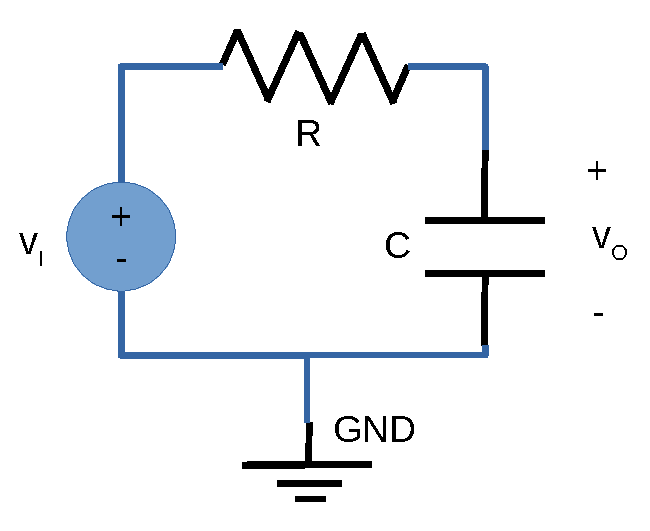
\includegraphics[width=0.4\linewidth]{rc.pdf}
\caption{Voltage driven serial RC circuit.}
\label{fig:rc}
\end{figure}


\section{Theoretical Analysis}
\label{sec:analysis}

\begin{equation}
    i_c = C \frac{dv_c}{dt}
    \label{eq:KVL}
\end{equation}

\subsection{Mesh Analysis}

\par The mesh method applies Kirchhoff's Voltage Law, Eq.\ref{eq:KVL}, to all circuit meshes, except ones containing current sources, after stipulating mesh current directions. A equation can be derived for each mesh, making use of Ohm's Law when needed, Eq. \ref{eq:Ohm}, forming an equation system. For meshes containing current sources, an equation can be obtained by inspection.

\begin{multicols}{2}
\begin{equation}
    \sum_{i=1}^{n} V_i = 0
    \label{eq:KVL}
\end{equation}

\begin{equation}
    V = I \times R
    \label{eq:Ohm}
\end{equation}
\end{multicols}

Below, we ilustrate the stipulated current directions for all meshes and components, in figure \ref{fig:figmesh}, and present the derived equation system in matrix form.


\begin{figure}[H]
  \centering
  \includegraphics[width=10cm]{../doc/MeshAnalysis}
  \caption{Circuit with current directions}
  \label{fig:figmesh}
\end{figure}

\begin{equation*}
\begin{bmatrix} R_1+R_3+R_4 & -R_3 & -R_4 & 0 \\
 -R_4 & 0 & R_4+R_6+R_7-K_c & 0 \\
 -K_bR_3 & K_bR_3-1 & 0 & 0 \\
 0 & 0 & 0 & -1 \end{bmatrix} \begin{bmatrix} I_{\alpha}\\ I_{\beta}\\ I_{\gamma} \\ I_{\delta} \end{bmatrix} = \begin{bmatrix} V_a\\ 0\\ 0\\ I_d \end{bmatrix}
\end{equation*}
%R_1+R_2+R_3 -R_3 -R_4 0
%-R_4 0 R_4+R_6+R_7-K_c 0
%-1 0 1-1/(K_bR_3) 0
%0 0 0 1

\par The first two equations were derived applying KVL to meshes $\alpha$ and $\gamma$, respectively. The third equation regards the inspection of dependent source $I_b$, and the forth equation is trivially obtained.
Analysing the matrix, one can quickly notice that $\alpha$, $\beta$ and $\gamma$ mesh currents are independent of source current $I_d$.

\par The matrix system was solved using Octave software. The results for mesh currents were used to calculate all branch currents, the latter being presented in the table below. This way results can be more easily compared between sections.



\begin{table}[H]
  \centering
  \begin{tabular}{|l|r|}
    \hline
    {\bf Name} & {\bf Value [A]} \\ \hline
    %\input{../mat/data_octave_current}
  \end{tabular}
  \caption{Theoretical Values for currents using Octave}
  \label{tab:TCurrents}
\end{table}

\subsection{Node Analysis}
\par The nodal method applies Kirchhoff's Current Law, Eq.\ref{eq:KCL}, to all circuit nodes, except ones next to voltage sources. A equation can be derived for each node, using Ohm's Law when needed, Eq. \ref{eq:Ohm}, forming a equation system. Usually, the ground node is stipulated next to a voltage source, so that two nodal voltages can be directly inferred. If there is more than one voltage source, which is our case, one can write additional equations considering the so called "supernode", which is the analysis of two consecutive nodes as one, and applying KCL only to external branches. In the presence of dependent voltage sources, one can also derive a equation from inspection.
\begin{multicols}{2}
\begin{equation}
    \sum_{i=1}^{n} I_i = 0
    \label{eq:KCL}
\end{equation}

\begin{equation}
    G = \frac{1}{R}
    \label{eq:G}
\end{equation}
\end{multicols}

Below, we illustrate the stipulated voltage directions for all branches, in figure \ref{fig:fignode}, and present the derived equation system in matrix form. For a practical purpose, we expressed the resistances as their equivalent conductances, as related by Eq.\ref{eq:G}.


\begin{figure}[H]
  \centering
  \includegraphics[width=10cm]{../doc/NodeAnalysis}
  \caption{Circuit with numbered nodes}
  \label{fig:fignode}
\end{figure}


\begin{equation*}
\begin{bmatrix}
 1 & 0 & 0 & 0 & 0 & 0 & 0 \\
 G_1 & -G_1 & 0 & 0 & 0 & -G_6 & -G_4 \\
 -G_1 & G_1+G_2+G_3 & -G_2 & 0 & 0 & 0 & -G_3\\
 0 & G_2+K_b & -G_2 & 0 & 0 & 0 & -K_b\\
 0 & -K_b & 0 & -G_5 & 0 & 0 & K_b+G_5\\
 0 & 0 & 0 & 0 & -1 & K_cG_6 & 1\\
 0 & 0 & 0 & 0 & -G_7 & G_6+G_7 & 0\end{bmatrix}
\begin{bmatrix}
 V_1\\ V_2\\ V_3\\ V_4\\ V_5\\ V_6\\ V_7\end{bmatrix}
=
\begin{bmatrix}
 V_a\\ 0\\ 0\\ 0\\ -I_d\\ 0\\ 0 \end{bmatrix}
\end{equation*}

\par The first equation is trivially inferred. The second equation is derived from considering nodes 0 and 1 as a supernode. Equations 3 up to 5 regard the application of KCL to nodes 2 up to 4, as well as the seventh equation comes from node 6. Finally, equation 6 comes from inspection of dependent source $V_c$. The supernode surrounding $V_c$ could also be considered.

\par The matrix system was solved using Octave software. The results for node voltages are presented in the table below.


\begin{table}[H]
  \centering
  \begin{tabular}{|l|r|}
    \hline
    {\bf Name} & {\bf Value [V]} \\ \hline
    %\input{../mat/data_octave_tensoes}
  \end{tabular}
  \caption{Theoretical values for node voltages using Octave}
  \label{tab:TVoltages}
\end{table}


\section{Simulation Analysis}
\label{sec:simulation}

\subsection{Operating Point Analysis}

In order to input the given circuit into the simulation software, \emph{ngspice}, we proceeded to number the existing nodes. It is fundamental to specify to which nodes each component is connected to, carefully distinguishing the positive from the negative terminal, once that this is going to affect the current value returned.

\emph{Ngspice} measures the voltages in each node and the current through any voltage source. In order to define $V_c$ one needs to have access to the current going through $R_6$. We have achieved this by adding a voltage source $V_{aux}$, with voltage $0V$, in series with $R_6$ and taking its current, since this is the same for components in series. Voltage source, $V_{aux}$, is, therefore connected to terminals 0 and 8, where 8 is a terminal located between $R_6$ and node 0.

\begin{figure}[H]
  \centering
  \includegraphics[width=10cm]{../doc/NGSpice}
  \caption{Considered circuit to input in \emph{ngspice}}
  \label{fig:fignodos}
\end{figure}

After inputing all components into \emph{ngspice}, we then ran the simulation program printing the current going through every component and the voltages in every node.


Table \ref{tab:ngspice} shows the simulated results for the circuit
under analysis.

\begin{table}[H]
  \centering
  \begin{tabular}{|l|r|}
    \hline
    {\bf Name} & {\bf Value [A or V]} \\ \hline
    @cb[i] & 0.000000e+00\\ \hline
@ce[i] & 0.000000e+00\\ \hline
@q1[ib] & 7.022567e-05\\ \hline
@q1[ic] & 1.404513e-02\\ \hline
@q1[ie] & -1.41154e-02\\ \hline
@q1[is] & 5.765392e-12\\ \hline
@rc[i] & 1.411536e-02\\ \hline
@re[i] & 1.411536e-02\\ \hline
@rf[i] & 7.022567e-05\\ \hline
@rs[i] & 0.000000e+00\\ \hline
v(1) & 0.000000e+00\\ \hline
v(2) & 0.000000e+00\\ \hline
base & 2.254108e+00\\ \hline
coll & 5.765392e+00\\ \hline
emit & 1.411536e+00\\ \hline
vcc & 1.000000e+01\\ \hline

  \end{tabular}
  \caption{Operating point analysis. A variable preceded by @ is of type {\em current}
    and expressed in Ampere; other variables are of type {\it voltage} and expressed in
    Volt.}
  \label{tab:ngspice}
\end{table}

One can immediately notice that current values for the voltage sources are approximately symmetrical to the ones presented in the theoretical analysis. This is because we have considered the current in the voltage sources going from the negative terminal to the positive one. On the other hand, \emph{ngspice} considers the current the other way around, i.e., entering the positive terminal.


%formula do erro
\begin{equation}
  \centering
  \epsilon (x_e)=\frac{|x_e-x_r|}{x_r} \times 100\,\%
  \label{eq:error}
\end{equation}

We have considered the value obtained by the mashes/nodes methods as the "real" one ($x_r$) and the value obtained through \emph{ngspice} as the experimental one ($x_e$). It is important to notice, once more, that the values from \emph{ngspice} for the current going through the voltages sources are simetric to the ones we have considered. The percentual error computation had this in mind.

Here, we present the obtained values for the errors.

\begin{table}[H]
  \centering
  \begin{tabular}{|l|r|}
    \hline
    {\bf Name} & {\bf Value in \%} \\ \hline
    \input{../mat/error_tensoes}
  \end{tabular}
  \caption{Voltages' percentual errors}
  \label{tab:error_tensoes}
\end{table}



\begin{table}[H]
  \centering
  \begin{tabular}{|l|r|}
    \hline
    {\bf Name} & {\bf Value in \%} \\ \hline
    \input{../mat/error_current}
  \end{tabular}
  \caption{Currents' percentual errors }
  \label{tab:error_current}
\end{table}

We have not considered the error in the $8^{th}$ node, once that it is defined to be exactly 0. Therefore, the use of equation \ref{eq:error} would give us an infinite answer. However, we have presented the error for $V_a$. Although this voltage was given to us by the \emph{python} code available, \emph{ngspice} is unable to consider the same number of significant figures as the ones presented, resulting in a non-zero value.





\section{Conclusion}
\label{sec:conclusion}

[argue output DC level deviation, voltage ripple, cost, accuracy/discrepancy, merit]



Comparing the results obtained in the theoretical analysis  with the ones acquired from \textit{ngspice} and also checking the \textit{Octave} plots with the simulation's plots, we can say that they present (...)

The DC level deviation is [XX]$V$ in the simulation, [XX] orders of magnitude smaller than the DC level, which is (considerably good).
The same can be said of the voltage ripple (...)

[accuracy/discrepanc considerations]

The total cost of the circuit is [XX] monetary units. The established cost of components obviously favours the use of diodes, which was our choise, allowing a relatively low total cost.  

With all the measurements and figures presented, we calculated the merit figure of our designed circuit as [XX].

%significantly small errors, mainly derived from precision limitations. We can thus conclude
% that our theoretical analysis matches the simulated circuit and can effectively describe the system's voltages and currents in stationary regimes,
% their time evolution and their frequency dependence, proving that it represents a really good approximation of reality.

% \par

% The operating point analyses match because \textit{ngspice} works by solving a matrix of linear equations based on the Kirchhoff's Laws, much like
% what we do on the theoretical analysis. The transient analyses also match because the differential equations that rule the system's behaviours have
% explicit solutions, and we can easily apply these solution, having only to take precautions with the initial conditions. \textit{Ngspice} solves these
% differential equations numerically after we declare the initial conditions. Naturally, since the initial conditions found in the operating point analysis match,
% the transient analyses must match as well. In the frequency analysis, \textit{ngspice} simulates the steady-state solution of the system for multiple frequencies.
% This is what we essentially do in the theoretical analysis, exploiting the phasor notation for each frequency, which assumes that steady-state solution for the component's currents and node
% voltages all oscillate with the same frequency as the voltage source.

%\cleardoublepage

% ----------------------------------------------------------------------
%  Bibliography
% ----------------------------------------------------------------------
%\addcontentsline{toc}{section}{\bibname}
%\bibliographystyle{abbrvunsrtnat} % <<<<< SELECT IF USING REFERENCES BY NUMBER (CITATION ORDER)
%\bibliography{../../../BIBfile.bib}

% ----------------------------------------------------------------------
\end{document}
% ----------------------------------------------------------------------
